\begin{center}
  \section[Brain-Inspired Neuromorphic Processors]{\capitalisewords{Brain-Inspired Neuromorphic Processors for Energy-Efficient Artificial Intelligence Systems}}
  Ayan Deb, 3$^{rd}$ Year, ECE
\end{center}

\setcounter{figure}{0}
\setcounter{table}{0}

\begin{multicols}{2}
  \begin{abstract}
    \bfseries
    Artificial Intelligence (AI) has demonstrated significant potential in solving complex problems across science, engineering, finance, healthcare, transportation, and education. However, conventional general-purpose processors based on the von Neumann architecture face the \textquotedblleft memory wall\textquotedblright{} problem when used for modern AI workloads. Deep Neural Networks (DNNs) can achieve high accuracy, but their heavy matrix operations, frequent memory access, and large computational requirements make them unsuitable for many real-time, edge, and embedded applications.

    \noindent
    Neuromorphic computing addresses these limitations by imitating the event-driven operation and neuron--synapse organization of the human brain. Spiking Neural Networks (SNNs) process information through sparse electrical events and can be implemented on low-power processors such as Intel Loihi, IBM TrueNorth, and SpiNNaker. This report reviews neuromorphic circuit design, SNN foundations, efficient model evaluation, Neural Architecture Search (NAS), hybrid DNN--SNN systems, and the signal-integrity considerations associated with heterogeneous CMOS- and memristor-based hardware.

    \noindent
    The report also examines a hybrid architecture in which conventional DNN layers perform feature extraction while a neuromorphic SNN performs event-driven inference. Such systems seek to preserve the accuracy of deep learning while reducing energy consumption, processing latency, and memory-transfer overhead. Their wider adoption will depend on improved training algorithms, scalable hardware, standardized software frameworks, and reliable integration with sensors and memory technologies.

    \vspace{1em}
    {\justifying\noindent\textbf{Keywords:} Neuromorphic Computing, Spiking Neural Networks, Deep Neural Networks, Neural Architecture Search, Signal Integrity, Heterogeneous Integration, Energy-Efficient Computing, Edge AI.\par}
  \end{abstract}

  \subsection*{\centering\uppercase{Introduction}}
  Artificial Intelligence was formally established as a field during the Dartmouth Conference of 1956 [1]. Since then, AI has developed into a widely used technology capable of imitating and extending aspects of human intelligence. Its applications now include medical diagnosis, autonomous transportation, industrial automation, communication systems, financial analysis, and scientific research.

  \noindent
  Most conventional computing platforms use the von Neumann architecture, in which processing and memory are physically separated. AI workloads require data to move repeatedly between these units, producing a communication bottleneck known as the \textbf{memory wall} [3]. Graphics Processing Units (GPUs), Field-Programmable Gate Arrays (FPGAs), and Application-Specific Integrated Circuits (ASICs) accelerate computation, but they still consume significant energy when processing large neural networks.

  \noindent
  The human brain provides a radically different computing model. It contains more than \(10^{11}\) neurons and approximately \(10^{15}\) synaptic connections, yet operates using roughly \(20\,\mathrm{W}\) of power. Inspired by this efficiency, researchers have developed neuromorphic chips that reproduce selected characteristics of biological neural systems, including event-driven signaling, local memory, parallel processing, and adaptive synaptic connections [2].

  \noindent
  Spiking neuromorphic chips implement SNNs, which are often described as the third generation of neural-network models [5]. They transmit information only when a neuron generates a spike, allowing inactive parts of the system to consume very little dynamic energy. This spatiotemporal representation can provide low latency, high processing speed, and energy-efficient operation for suitable workloads [6]. Nevertheless, future systems must imitate neural behavior more effectively and address communication, integration, and signal-integrity challenges.

  \subsection*{\centering\uppercase{Related Works}}
  Deep Neural Networks are widely used because they can learn complex patterns and achieve strong performance in image recognition, language processing, healthcare, and intelligent transportation [7]. Their accuracy, however, is supported by intensive multiply--accumulate operations and large memory requirements. These characteristics increase energy consumption and restrict the deployment of advanced DNNs on real-time and resource-constrained devices.

  \noindent
  Neuromorphic Computing (NC) offers an alternative by using SNNs and event-driven hardware. Platforms such as Intel Loihi and IBM TrueNorth have demonstrated low-power processing for robotics, sensing, and embedded AI [8], [9]. Hybrid systems that combine DNN feature extraction with SNN-based inference have therefore become an important research direction, since they aim to combine DNN accuracy with neuromorphic efficiency [10], [11].

  \noindent
  Neural Architecture Search automatically develops neural-network structures instead of relying entirely on manual design [12], [13]. NAS techniques include reinforcement learning, gradient-based optimization, Genetic Algorithms (GAs), and Particle Swarm Optimization (PSO). Evolutionary NAS can reduce the computational burden of architecture discovery by progressively selecting and refining high-performing candidates [14]--[18]. Combining NAS with neuromorphic computing may produce SNN architectures that are better matched to event-driven hardware.

  \subsection*{\centering\uppercase{Research Methodology}}
  The proposed research methodology begins by identifying the computational inefficiencies and high power consumption of conventional deep-learning architectures. A hybrid DNN--NC model is then constructed by retaining dense layers for feature extraction and converting selected processing stages into spiking layers. The objective is to reduce the number of energy-intensive operations while maintaining a practical balance among classification accuracy, processing speed, and energy efficiency.

  \noindent
  Input data first undergoes preprocessing before being passed to the DNN feature extractor. Extracted features are encoded into spike trains and processed by an event-driven SNN. The hybrid model is then evaluated using accuracy, power consumption, latency, and computational-efficiency measurements. Results from the neuromorphic implementation are compared with those of a conventional GPU- or TPU-based model.

  \begin{center}
\vspace{-0.5em}
\begin{minipage}{0.98\columnwidth}
\centering
    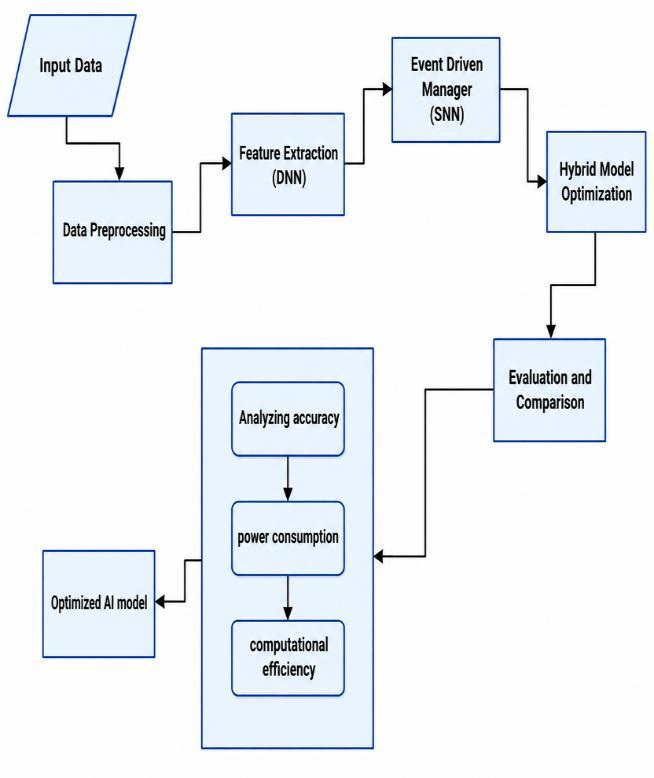
\includegraphics[width=0.72\columnwidth]{assets/images/ayan_brain_architecture.jpg}
    \captionof{figure}{Architecture of the proposed brain-inspired hybrid computing workflow.}
\end{minipage}
  \end{center}
\vspace{-0.35em}

  \subsection*{\centering\uppercase{Efficient Evaluation}}
  During evolutionary architecture search, the performance of each candidate model must be evaluated before the next generation can be produced. Training every candidate network from scratch until convergence can require many GPU-days [19]--[21]. Model evaluation consequently becomes the most time-consuming stage of the optimization process.

  \noindent
  Efficient evaluation methods reduce this cost by estimating candidate performance with less training. These approaches are commonly divided into \textbf{few-shot}, \textbf{one-shot}, and \textbf{zero-shot} evaluation. Few-shot methods train candidates for a limited number of steps, one-shot methods share parameters through a common supernetwork, and zero-shot methods use inexpensive indicators to rank architectures without full training. Such techniques make evolutionary optimization more practical for SNNs and hybrid models.

  \subsection*{\centering\uppercase{SNN Foundation}}
  In an SNN, presynaptic neurons transmit information using discrete spikes. A postsynaptic neuron integrates these incoming events and emits its own spike when the accumulated membrane potential reaches a threshold. This report adopts the widely used \textbf{Leaky Integrate-and-Fire (LIF)} neuron model [22].

  \noindent
  The membrane potential begins near a resting value \(V_{\mathrm{rest}}\). Incoming spikes increase the potential, while a leakage mechanism causes it to decay over time. When the potential reaches the firing threshold \(V_{\mathrm{th}}\), the neuron produces a spike and returns to its resting state. Because computation occurs mainly when events arrive, LIF-based systems can substantially reduce unnecessary activity.

  \begin{center}
\vspace{-0.5em}
\begin{minipage}{0.98\columnwidth}
\centering
    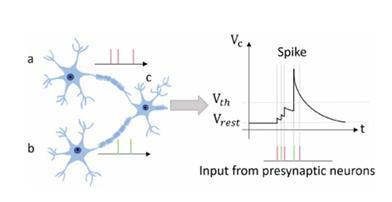
\includegraphics[width=0.75\columnwidth]{assets/images/ayan_lif_neuron.jpg}
    \captionof{figure}{Computation of an LIF neuron receiving spikes from presynaptic neurons.}
\end{minipage}
  \end{center}
\vspace{-0.35em}

  \noindent
  The architecture-search process represents an SNN using a genotype that encodes modules, neural motifs, and inter-module connections. The phenotype is the resulting executable network. Local modules are inspired by recurring neural circuits, while global cross-module connections permit information to move between distant parts of the model. This combination allows architecture evolution to explore structures beyond direct copies of conventional DNNs.

  \begin{center}
\vspace{-0.5em}
\begin{minipage}{0.98\columnwidth}
\centering
    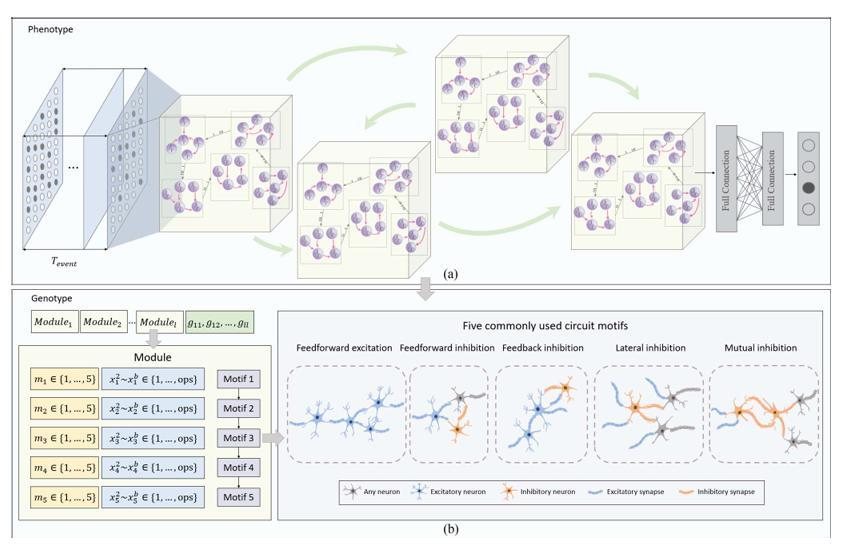
\includegraphics[width=0.85\columnwidth]{assets/images/ayan_snn_encoding.jpg}
    \captionof{figure}{Phenotype-to-genotype mapping using modular neural circuits and global connectivity.}
\end{minipage}
  \end{center}
\vspace{-0.35em}

  \subsection*{\centering\uppercase{Model Architecture and Training Protocols}}
  The hybrid model combines conventional dense processing with a spiking inference stage. Its DNN section contains three fully connected layers with 128, 64, and 32 neurons using Rectified Linear Unit (ReLU) activation. The neuromorphic section contains an SNN with 100 spiking neurons and Spike-Timing-Dependent Plasticity (STDP) learning.

  \noindent
  Input features are converted into spike trains through rate coding. Training uses the Adam optimizer with a learning rate of \(0.001\), a batch size of 32, and a maximum of 50 epochs. Early stopping limits overfitting, while data augmentation and dropout regularization with a rate of \(0.3\) improve generalization. Spike thresholds are optimized for efficient execution on the Intel Loihi framework.

  \subsection*{\centering\uppercase{Comparison with Traditional Deep Learning Architectures}}
  The hybrid system must be evaluated against an equivalent conventional deep-learning model. Accuracy indicates whether conversion to spiking computation preserves useful predictive performance. Energy savings can be expressed as the percentage reduction in power consumption, while computational cost measures processing time, operation count, latency, and memory traffic.

  {\justifying\noindent
  Traditional DNN accelerators provide high throughput for dense numerical operations, but their energy use increases with model size and repeated memory access. Neuromorphic hardware can be more efficient when inputs are sparse and event-driven. Its benefit is therefore workload-dependent: dense tasks may continue to favor GPUs or TPUs, whereas sensing, robotics, and edge applications may benefit from spike-based computation.\par}

  \subsection*{\centering\uppercase{Deep Neural Networks}}
  A Deep Neural Network is an artificial neural network containing multiple processing layers between its input and output. DNNs are constructed from neurons, weighted connections, biases, and nonlinear activation functions. Training adjusts the weights so that the network can approximate complex relationships in data [23].

  \noindent
  DNNs provide strong accuracy and mature training methods, but they generally process continuous numerical values at every layer. This produces large numbers of operations even when the input contains little new information. Their dependence on memory bandwidth and parallel arithmetic contributes to the energy cost of modern AI.

  \subsection*{\centering\uppercase{Neuromorphic Computing}}
  Neuromorphic computing uses specialized circuits and algorithms to imitate selected structural and operational principles of the brain. Memory and computation are placed close together, communication is event-driven, and SNN neurons exchange discrete spikes. These characteristics reduce data movement and allow inactive circuits to remain idle.

  \noindent
  Neuromorphic processors are particularly suitable for edge devices, where power, latency, and physical size are constrained. Hardware such as Intel Loihi, IBM TrueNorth, and SpiNNaker demonstrates the feasibility of scalable brain-inspired computation. Neuromorphic systems may also provide fault tolerance and adaptive learning, although programming tools and deployment standards remain less mature than those available for conventional deep learning.

  \begin{center}
\vspace{-0.5em}
\begin{minipage}{0.98\columnwidth}
\centering
    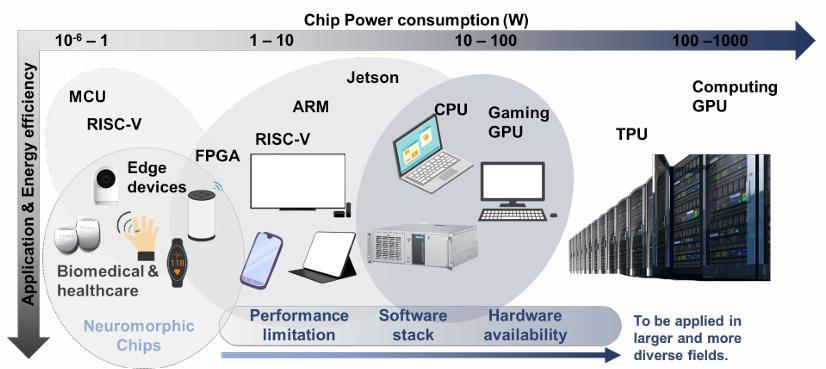
\includegraphics[width=0.85\columnwidth]{assets/images/ayan_neuromorphic_applications.jpg}
    \captionof{figure}{Neuromorphic processors occupy the low-power edge of the AI hardware landscape.}
\end{minipage}
  \end{center}
\vspace{-0.35em}

  \subsection*{\centering\uppercase{Hybrid Deep Learning and Neuromorphic Computing for Energy-Efficient AI}}
  Hybrid AI combines the high accuracy of DNNs with the energy efficiency of neuromorphic processing. Selected DNN layers can be converted into SNN stages and deployed on event-driven hardware such as Intel Loihi or SpiNNaker. The conventional portion of the model performs feature extraction, while the spiking portion handles sparse inference or temporal processing.

  \noindent
  This approach can reduce power consumption and latency for edge AI, robotics, Internet of Things devices, and always-on sensing. It also avoids the need to replace the entire deep-learning pipeline at once. However, effective conversion requires careful spike encoding, threshold optimization, accuracy preservation, and hardware-aware training.

  \begin{center}
\vspace{-0.5em}
\begin{minipage}{0.98\columnwidth}
\centering
    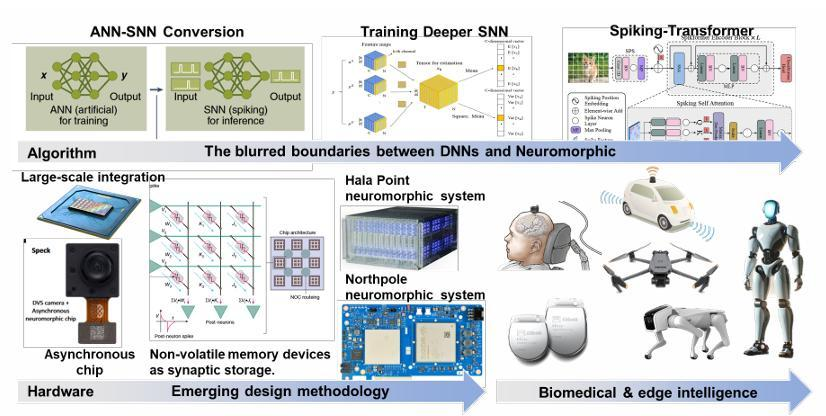
\includegraphics[width=0.85\columnwidth]{assets/images/ayan_trends.jpg}
    \captionof{figure}{Trends in neuromorphic algorithms, chips, memory technologies, and edge applications.}
\end{minipage}
  \end{center}
\vspace{-0.35em}

  \subsection*{\centering\uppercase{Conclusion and Future Scope}}
  Neuromorphic computing offers a promising approach to energy-efficient AI by replacing continuous, clock-driven processing with sparse, event-driven computation. SNNs and LIF neurons provide a foundation for brain-inspired hardware, while NAS and evolutionary optimization can discover architectures that are better suited to neuromorphic execution.

  \noindent
  Current SNN research still relies heavily on fixed structures derived from DNNs, and many NAS-based SNN models do not yet consistently outperform carefully designed conventional networks. Future work should therefore improve SNN training accuracy, develop faster evaluation strategies, and evolve architectures using modular neural motifs and long-range connections.

  \noindent
  Progress in hardware platforms such as Intel Loihi, IBM TrueNorth, and SpiNNaker can improve flexibility and computational efficiency. Hybrid models should also be tested in practical applications including healthcare diagnostics, autonomous vehicles, smart cities, industrial sensing, and robotics. Standardized frameworks for integrating DNNs with neuromorphic hardware will be essential for the large-scale adoption of energy-efficient, real-time AI systems.

  \subsection*{\centering\uppercase{References}}
  {\small
  \begingroup\justifying
  \Urlmuskip=0mu plus 1mu\relax
  \begin{enumerate}[leftmargin=*,itemsep=0.20em]
    \item J. McCarthy, M. L. Minsky, N. Rochester, et al., “A proposal for the Dartmouth summer research project on artificial intelligence, August 31, 1955,” \textit{AI Magazine}, vol. 27, no. 4, pp. 12--14, 2006.
    \item W. Q. Zhang, B. Gao, J. S. Tang, et al., “Neuro-inspired computing chips,” \textit{Nature Electronics}, vol. 3, no. 7, pp. 371--382, 2020.
    \item A. Krikelis and C. C. Weems, “Associative processing and processors,” \textit{Computer}, vol. 27, no. 11, pp. 12--17, 1994.
    \item J. Pei, L. Deng, S. Song, et al., “Towards artificial general intelligence with hybrid Tianjic chip architecture,” \textit{Nature}, vol. 572, no. 7767, pp. 106--111, 2019.
    \item W. Maass, “Networks of spiking neurons: The third generation of neural network models,” \textit{Neural Networks}, vol. 10, no. 9, pp. 1659--1671, 1997.
    \item A. Reuther, P. Michaleas, M. Jones, et al., “AI and ML accelerator survey and trends,” in \textit{Proceedings of the 2022 IEEE High Performance Extreme Computing Conference}, Waltham, MA, USA, pp. 1--10, 2022.
    \item G. I. Okolo, S. Katsigiannis, and N. Ramzan, “IEViT: An enhanced vision transformer architecture for chest X-ray image classification,” \textit{Computer Methods and Programs in Biomedicine}, vol. 226, p. 107141, Nov. 2022, doi: 10.1016/j.cmpb.2022.107141.
    \item S. Liu, J. Yu, X. Deng, and S. Wan, “FedCPF: An efficient communication federated learning approach for vehicular edge computing in 6G communication networks,” \textit{IEEE Transactions on Intelligent Transportation Systems}, vol. 23, no. 2, pp. 1616--1629, Feb. 2022, doi: 10.1109/TITS.2021.3099368.
    \item Z. Dong, X. Ji, G. Zhou, M. Gao, and D. Qi, “Multimodal neuromorphic sensory-processing system with memristor circuits for smart home applications,” \textit{IEEE Transactions on Industry Applications}, vol. 59, no. 1, pp. 47--58, Jan. 2023, doi: 10.1109/TIA.2022.3188749.
    \item “A fast and energy-efficient SNN processor with adaptive clock/event-driven computation scheme and online learning,” \textit{IEEE Xplore}. [Online]. Available: \url{https://ieeexplore.ieee.org/abstract/document/9336327}.
    \item “Edge-based collaborative training system for Artificial Intelligence of Things,” \textit{IEEE Xplore}. [Online]. Available: \url{https://ieeexplore.ieee.org/abstract/document/9699416}.
    \item T. Elsken, J. H. Metzen, and F. Hutter, “Neural architecture search: A survey,” \textit{Journal of Machine Learning Research}, vol. 20, no. 1, pp. 1997--2017, 2019.
    \item G. Ghiasi, T.-Y. Lin, and Q. V. Le, “NAS-FPN: Learning scalable feature pyramid architecture for object detection,” in \textit{Proceedings of the IEEE/CVF Conference on Computer Vision and Pattern Recognition}, pp. 7036--7045, 2019.
    \item B. Zoph and Q. V. Le, “Neural architecture search with reinforcement learning,” arXiv:1611.01578, 2016.
    \item P. Ren et al., “A comprehensive survey of neural architecture search: Challenges and solutions,” \textit{ACM Computing Surveys}, vol. 54, no. 4, pp. 1--34, 2021.
    \item K. Price, R. M. Storn, and J. A. Lampinen, \textit{Differential Evolution: A Practical Approach to Global Optimization}. New York, NY, USA: Springer-Verlag, 2006.
    \item Y. Sun, G. G. Yen, and Z. Yi, “IGD indicator-based evolutionary algorithm for many-objective optimization problems,” \textit{IEEE Transactions on Evolutionary Computation}, vol. 23, no. 2, pp. 173--187, Apr. 2019.
    \item Z. Lu et al., “NSGA-Net: Neural architecture search using multi-objective genetic algorithm,” in \textit{Proceedings of the Genetic and Evolutionary Computation Conference}, pp. 419--427, 2019.
    \item E. Real, A. Aggarwal, Y. Huang, and Q. V. Le, “Regularized evolution for image classifier architecture search,” in \textit{Proceedings of the AAAI Conference on Artificial Intelligence}, vol. 33, no. 1, pp. 4780--4789, 2019.
    \item B. Zoph and Q. V. Le, “Neural architecture search with reinforcement learning,” arXiv:1611.01578, 2016.
    \item E. Real et al., “Large-scale evolution of image classifiers,” in \textit{Proceedings of the International Conference on Machine Learning}, PMLR, pp. 2902--2911, 2017.
    \item B. Nicolas, C. Mark, and W. van Rossum, “Quantitative investigations of electrical nerve excitation treated as polarization,” \textit{Biological Cybernetics}, vol. 97, no. 5--6, p. 341, 2007.
    \item “Deep learning,” \textit{Wikipedia}. [Online]. Available: \url{https://en.wikipedia.org/wiki/Deep_learning\#Deep_neural_networks}.
  \end{enumerate}
  \par\endgroup
  }
\end{multicols}